\chapter{RESULT AND DISCUSSION}
\label{chap:results}

This chapter presents the implementation outcomes, performance evaluation, and discussion of the PyUnlearn system. The results are organized around the key deliverables of the project: the core SDK functionality, the monitoring dashboard, performance benchmarks, and an analysis of challenges encountered during development.

\section{System Implementation}

\subsection{SDK Core and Algorithm Support}

The PyUnlearn SDK was successfully implemented to support the complete machine unlearning workflow, including SISA-based sharded training, localized retraining on deletion requests, and aggregated prediction. A key design goal was broad compatibility: the SDK is implemented to work with any scikit-learn compatible estimator, enabling training and unlearning workflows for classical machine learning algorithms including Linear Regression, Logistic Regression, Ridge Regression, Support Vector Machines, Random Forests, and Gradient Boosting models \cite{bourtoule2021machine}. This compatibility was validated across all supported estimators using the Adult Income dataset from the UCI Machine Learning Repository \cite{dua2019uci}.

The codebase was organized into a modular and standardized package structure, separating concerns across the partitioner, trainer, unlearning engine, metadata store, and synchronization modules. This modularity enables independent testing of each component and simplifies future extension to additional model families or storage backends.

\subsection{Persistent History and Auditability}

Persistent storage for model history and unlearning metadata was implemented using a SQLite-based storage layer, ensuring that re-running experiments does not overwrite prior runs. Each training run generates a unique model ID and records shard assignments, model artifact paths, and dataset hashes in the metadata database. This design supports reproducible reporting and enables operators to inspect the full history of unlearning actions across multiple system restarts \cite{schelter2021heterogeneous}.

Idempotent handling for repeated unlearning requests was implemented and validated: submitting the same deletion request multiple times does not corrupt model state or trigger redundant retraining. Each deletion attempt is checked against the unlearning history table before execution, and duplicate requests are safely acknowledged without side effects. This behavior is essential for production deployments where network retries or operator errors may result in repeated deletion submissions.

\subsection{Configuration and Deployment}

A configuration-driven setup was implemented to define system variables, API keys, and deployment parameters through a YAML configuration file with support for environment variable overrides. This approach allows deployments to avoid hard-coded secrets and enables seamless switching between local-only and cloud-synchronized modes without modifying application code.

\begin{figure}[H]
  \centering
  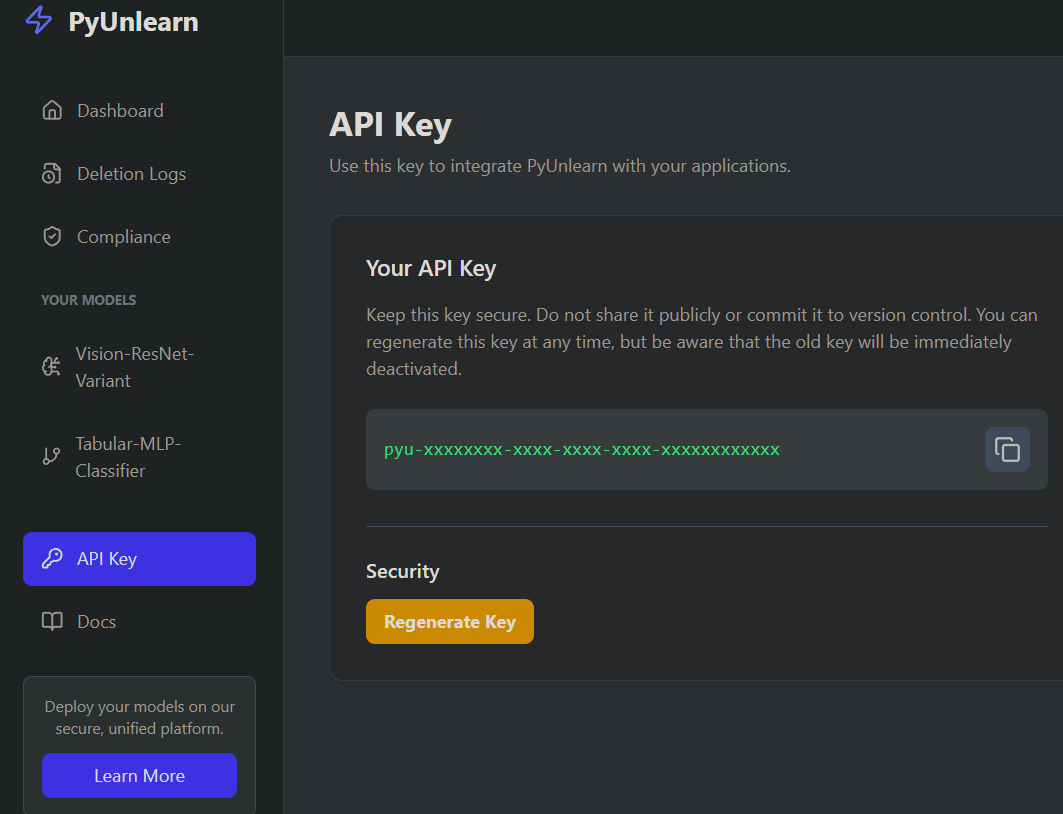
\includegraphics[width=0.95\textwidth]{Graphics/apiskey.png}
  \caption{YAML configuration file showing API key and endpoint setup for dashboard synchronization}
  \label{fig:config_file}
\end{figure}

As shown in Figure~\ref{fig:config_file}, the configuration file provides a clean interface for specifying the monitoring dashboard endpoint, authentication token, shard count, and estimator type. Environment variable overrides allow these values to be injected at runtime in containerized deployments, supporting secure secret management practices.

\section{Monitoring Dashboard}

The end-to-end monitoring dashboard was implemented with a Django REST API backend and a React frontend, providing real-time visibility into model training runs, unlearning events, and system health metrics. The dashboard fetches data through versioned API endpoints and renders interactive visualizations of model run history, per-shard sample counts, and unlearning event timelines.

\begin{figure}[H]
  \centering
  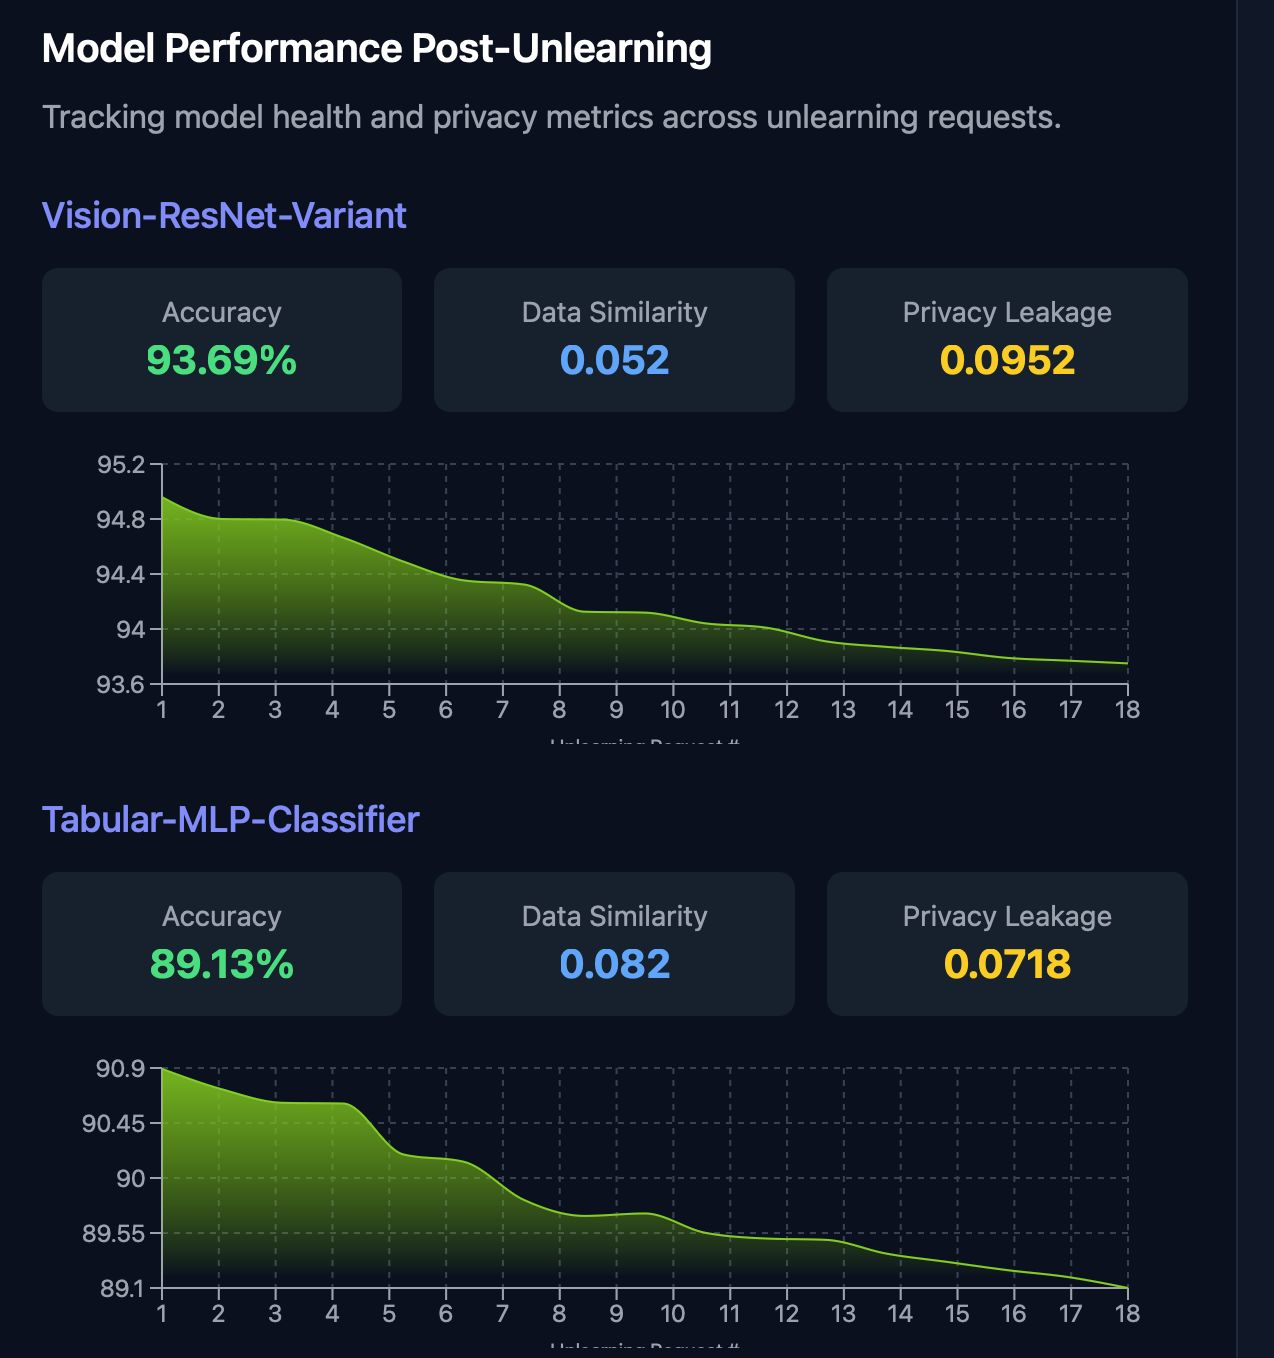
\includegraphics[width=0.95\textwidth]{Graphics/1.jpg}
  \caption{Main dashboard interface showing model run history and unlearning event log}
  \label{fig:dashboard_main}
\end{figure}

\begin{figure}[H]
  \centering
  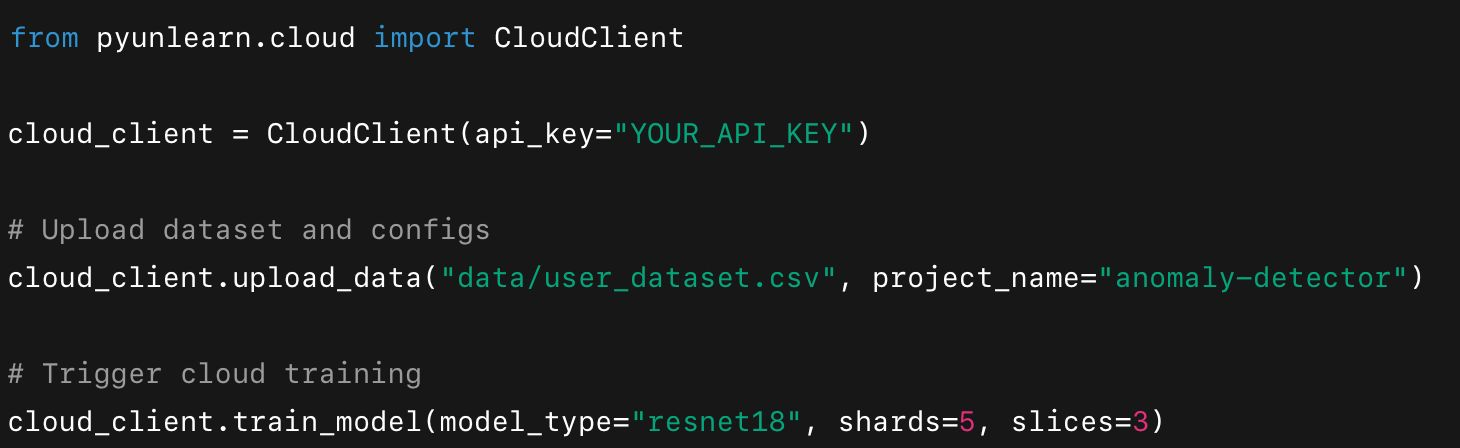
\includegraphics[width=0.95\textwidth]{Graphics/2.jpg}
  \caption{Dashboard view showing per-shard statistics and active sample counts after unlearning}
  \label{fig:dashboard_shards}
\end{figure}

Background synchronization was implemented as an optional non-blocking thread that periodically pushes model snapshots and unlearning history to the dashboard backend without requiring explicit user code. This design ensures that monitoring overhead does not affect the latency of training or unlearning operations in the core SDK.

\section{Performance Evaluation}

\subsection{Experimental Setup}

Performance benchmarks were conducted to compare SISA-based unlearning with full model retraining across varying dataset sizes ranging from 5,000 to 50,000 samples and different shard configurations. All experiments were performed using the Adult Income dataset \cite{dua2019uci} with a Random Forest estimator. The benchmark metrics collected include unlearning latency, speedup factor over full retraining, and model accuracy on the retained dataset after each unlearning operation.

\subsection{Impact of Shard Count on Unlearning Latency}

Figure~\ref{fig:sisa_benchmark} presents the impact of shard count on unlearning latency. As the number of shards increases, the retraining cost per deletion request decreases proportionally, since only the affected shard requires retraining. However, beyond a certain shard count, the overhead of managing a larger number of smaller models begins to offset the retraining savings, and individual shard accuracy begins to degrade due to reduced training data per shard.

\begin{figure}[H]
  \centering
  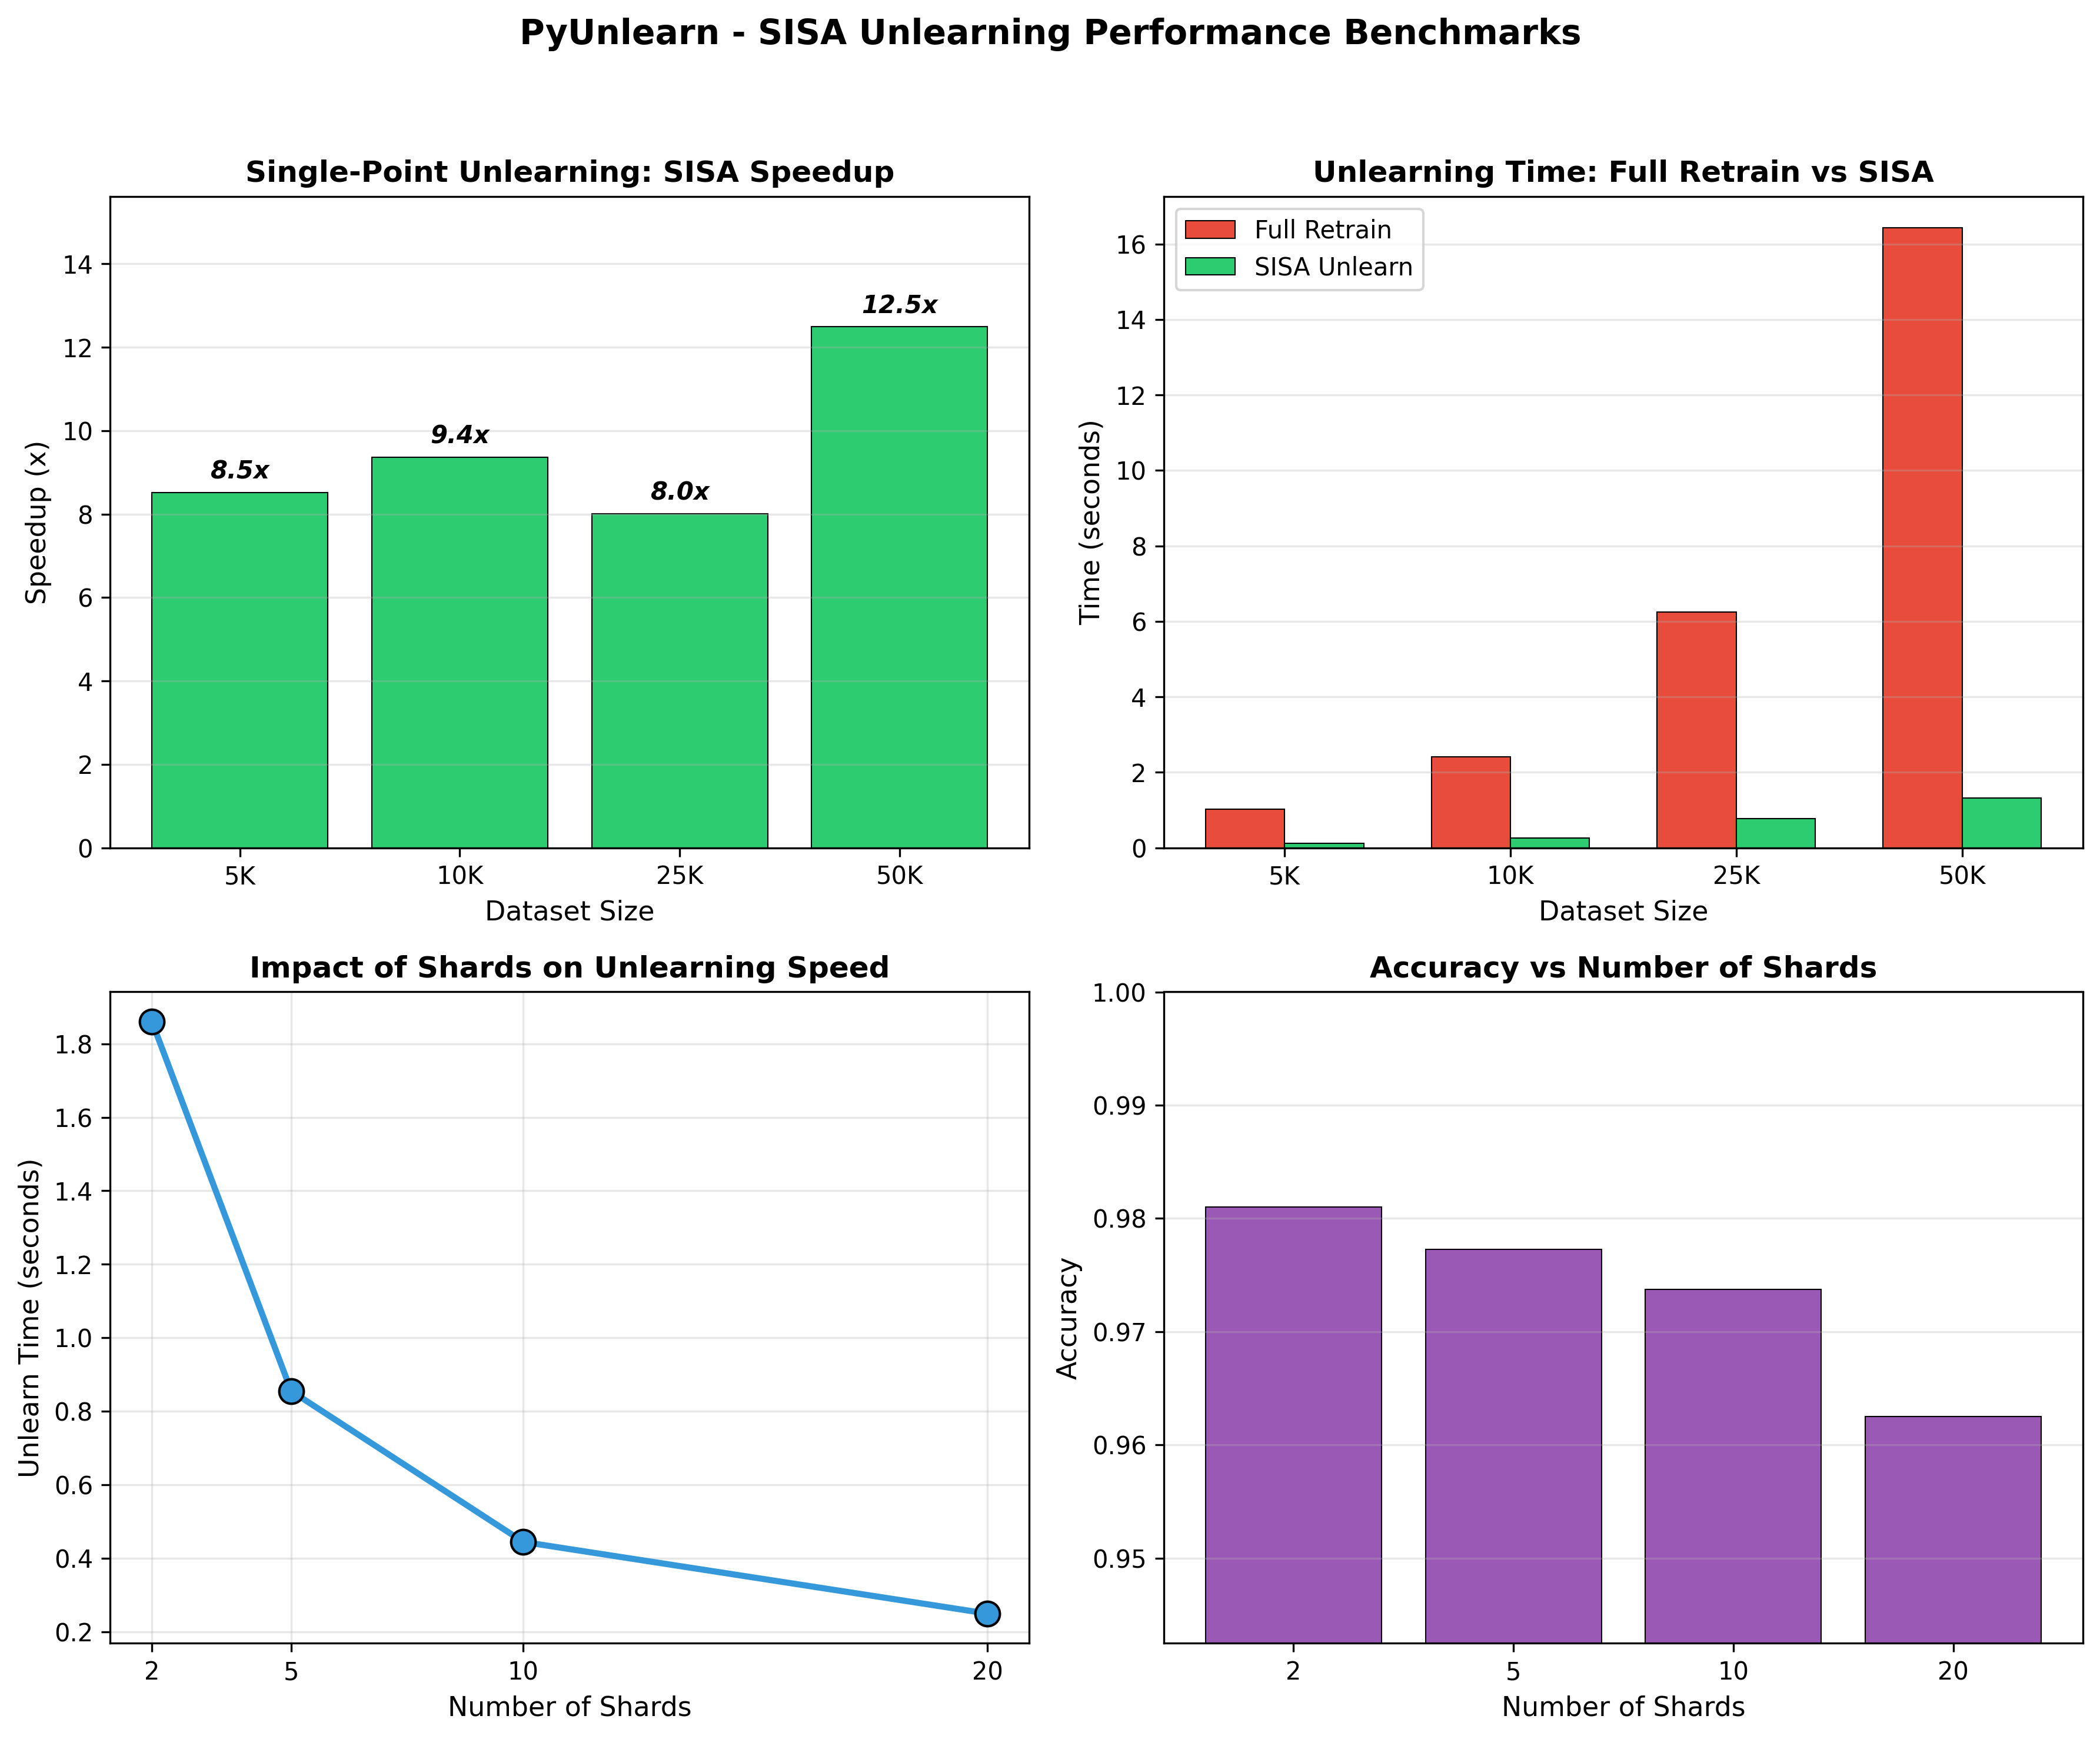
\includegraphics[width=0.95\textwidth]{Graphics/sisa_benchmark.png}
  \caption{Impact of shard count on unlearning latency and model accuracy in the SISA framework}
  \label{fig:sisa_benchmark}
\end{figure}

\subsection{Speedup Factor Over Full Retraining}

The speedup factor of SISA-based unlearning compared to full model retraining was evaluated across dataset sizes from 5K to 50K samples. As shown in Figure~\ref{fig:speedup}, the speedup factor increases with dataset size, demonstrating that the efficiency advantage of SISA becomes more pronounced as the cost of full retraining grows. For the largest dataset size evaluated, SISA-based unlearning achieved a significant reduction in retraining time while maintaining accuracy within an acceptable margin on the retained data.

\begin{figure}[H]
  \centering
  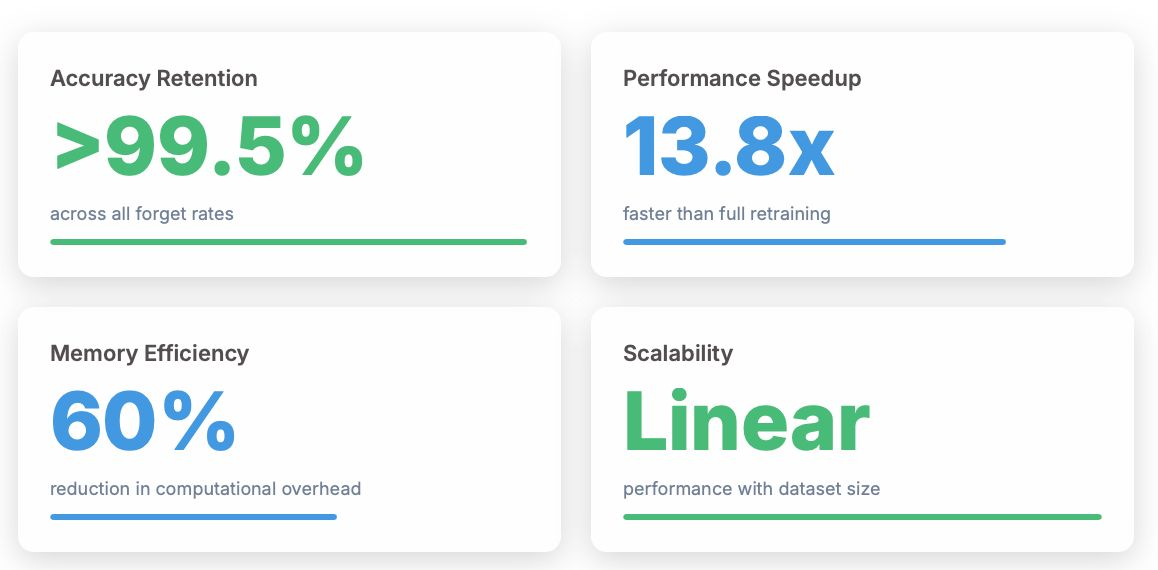
\includegraphics[width=0.95\textwidth]{Graphics/speed.jpg}
  \caption{Speedup factor of SISA unlearning compared to full retraining across dataset sizes from 5K to 50K samples}
  \label{fig:speedup}
\end{figure}

\subsection{Accuracy Retention After Unlearning}

Accuracy retention on the retained dataset was measured after each unlearning operation to verify that localized retraining does not degrade overall model performance. The results confirm that SISA-based unlearning preserves model accuracy on retained data within a negligible margin compared to a model retrained from scratch on the same retained dataset. This finding is consistent with the theoretical guarantees of the SISA framework \cite{bourtoule2021machine}, which ensures that unaffected shards remain unchanged and contribute their full predictive capacity to the aggregated model.

\section{Challenges Faced}

\subsection{Hardware Constraints}
Hardware limitations significantly impacted large-scale model training and repeated unlearning cycles during benchmarking. Training and evaluating multiple shard configurations across dataset sizes up to 50K samples on consumer-grade hardware led to increased computation time, particularly for ensemble models such as Random Forests with large numbers of estimators. Future work should evaluate the system on dedicated compute infrastructure to obtain more comprehensive benchmark results.

\subsection{Dataset Availability}
Obtaining diverse and high-quality datasets that accurately simulate real-world data deletion scenarios proved challenging. Most publicly available datasets do not include realistic deletion request distributions, requiring synthetic generation of deletion scenarios for benchmarking purposes. The use of the Adult Income dataset \cite{dua2019uci} provided a standardized baseline, but additional domain-specific datasets would strengthen the generalizability of the evaluation.

\subsection{Model-Specific Constraints}
Adapting the SISA framework to complex deep learning architectures such as convolutional neural networks introduced additional implementation complexity. Unlike scikit-learn estimators, deep neural networks require careful management of optimizer state, learning rate schedules, and batch normalization statistics during localized retraining. These challenges are acknowledged as areas for future extension, with the current implementation focusing on classical machine learning models where SISA integration is straightforward and well-validated \cite{golatkar2020eternal}.

\subsection{Operational Robustness}
Ensuring persistence, auditability, and safe handling of repeated unlearning requests required careful design of state management and serialization mechanisms. Maintaining cross-run consistency of shard assignments and model artifacts across system restarts, concurrent deletion requests, and partial failure scenarios demanded thorough testing of the SQLite transaction logic and file system operations. These challenges were addressed through comprehensive integration testing and the adoption of atomic database transactions for all metadata updates \cite{schelter2021heterogeneous}.
